%%=============================================================================
%% chapters/chapter1.tex — Introduction (final-defense version)
%%=============================================================================
\chapter{Introduction}
\label{ch:intro}

\section{Background and Motivation}
\label{sec:background}

Modern robotic systems are evolving from executing simple, pre-programmed
commands toward intelligent agents that perceive their surroundings, reason
about them, and provide services grounded in knowledge of their environment. A
central enabler of this transition is the three-dimensional (3D) representation
of the operating environment. Whereas early mobile robots operated on
two-dimensional (2D) occupancy grids sufficient for collision-free navigation on
a single plane, an increasing number of robotic tasks now extend into the
vertical dimension: a mobile manipulator must reason about the 3D pose of a
graspable object, an industrial lift must localize a ceiling-mounted
installation target, and an inspection robot must relate components distributed
across the full height of a facility. In such settings, the quality of the
underlying 3D representation directly bounds the range of operations a robot
can perform.

A purely geometric point cloud tells a robot where surfaces are, but not what
they are or how they relate to one another. To act intelligently, a robot must
additionally understand the identity, attributes, and relationships of the
objects and places that populate the space. This understanding is captured by a
semantic model: a structured representation that augments raw geometry with
meaning. A well-constructed 3D semantic model serves as a shared substrate for
heterogeneous downstream robots, increasingly mediated by a digital twin---a
continuously updated, machine-readable model of the physical environment that
multiple robots and services can consult, reason over, and update.

Constructing such a representation in practice requires progress along two
tightly coupled fronts. The first is 3D mapping: acquiring and registering point
clouds into a globally consistent map with human intervention minimized.
Industrial, plant, and construction sites are increasingly captured with
survey-grade terrestrial laser scanners (TLS) for as-built modeling and facility
management, because such scanners deliver millimeter-accurate, globally
registered geometry. However, a TLS such as the Leica BLK360 must remain
stationary for minutes per pose and does not register scans in real time.
Conventional frontier-based exploration algorithms assume continuous motion and
online registration and are therefore fundamentally incompatible with this
sensing modality; bridging autonomous exploration and stationary survey-grade
scanning is a prerequisite for the automation this dissertation pursues. The
second front is point cloud semantic modeling: transforming the acquired
geometric data into a structured representation that encodes what each element
means and how elements relate. Converting a raw survey-grade point cloud into a
queryable semantic model that robots can act upon still relies largely on manual
annotation.

Two conceptual gaps motivate this dissertation. First, many existing semantic
mapping frameworks are tied to specific sensor modalities, such as RGB-D
cameras, or assume pre-built static inputs, which limits scalability in
environments that change continuously during operation. Second, semantic
information tends to be generated as auxiliary annotation rather than as a
structured knowledge representation, making it difficult for downstream
services to query, reason over, verify, and extend it. Beyond these, three
practical challenges arise at the implementation level. State-of-the-art 3D
segmentation and open-vocabulary classification models exhibit insufficient
accuracy when applied directly to survey-grade industrial point clouds, so that
pipelines that propagate their labels downstream hand the robot confident
fictions. Language interfaces that answer questions about a scene from an
unvalidated label dump hallucinate facts that a robot would act on. Finally,
scene models are typically built once and abandoned: a re-scan either rebuilds
everything, losing the object identities that planners and logs refer to, or is
not integrated at all, even though real sites drift continuously.

\section{Research Objectives}
\label{sec:objectives}

The objective of this dissertation is to propose and validate an integrated
framework in which a survey-grade 3D-point-cloud-laser-based mapping robot
acquires 3D maps of unknown indoor environments with human intervention
minimized, transforms the acquired point clouds into a verified and maintainable
ontological semantic model through a fully automated semantic modeling and
database construction pipeline, and enables downstream robots to determine
spatial operations semantically on the same representation. To this end, the
research pursues five sub-objectives:

\begin{itemize}[leftmargin=2.2em,itemsep=2pt]
  \item (O1) Design a frontier-based autonomous exploration strategy coupled
        with a stop-and-scan sequence, in which the decision to halt and scan
        is made by an occlusion-aware coverage model computed on the live
        occupancy map, so that stationary survey-grade scanners can be driven
        autonomously with as few scans as genuine observation requires.
  \item (O2) Build an object-level 3D recognition backbone that operates
        directly on survey-grade colored point clouds---preprocessing,
        deterministic geometry-aware decomposition, and open-vocabulary
        provisional classification---whose reproducibility underwrites
        verification and change detection.
  \item (O3) Propose a fully automated semantic modeling pipeline that converts
        recognized objects and places into a confidence-aware ontological
        knowledge graph based on the Triplet Ontological Semantic Model (TOSM),
        in which every label is verified by multi-view vision--language-model
        (VLM) inference with automatic escalation, unresolved content is
        retained as explicitly unverified, identities are preserved across
        re-scans, and query answers are structurally gated.
  \item (O4) Derive from the same 3D semantic model the multilayer,
        robot-consumable representation that spatial operations at different
        heights require---a driving layer (occupancy grid and place layer for
        navigation), a manipulation work layer (verified object footprints and
        poses at reach height), and an overhead layer (ceiling-mounted
        structure recognized from the same scan)---together with a
        physics-enabled simulation stage, so that the representation remains
        compatible with conventional 2D-laser-based navigation stacks and
        with simulation-based commissioning.
  \item (O5) Validate the integrated framework through digital-twin integration
        and consumption by a physical spatial-operation robot---a mobile
        manipulator that drives on the driving layer, manipulates at work
        height, and can point its end effector at overhead targets---so that
        the console, the twin, and the robot act on one semantic store.
\end{itemize}

\section{Contributions}
\label{sec:contributions}

To meet these objectives, this dissertation proposes an end-to-end framework
that minimizes human intervention, organized into three parts
(Figure~\ref{fig:overall})---Part~A: 3D mapping with autonomous exploratory
acquisition; Part~B: fully automated point cloud semantic modeling; and Part~C:
digital-twin-based validation. The principal contributions are as follows.

\begin{enumerate}[leftmargin=2.2em,itemsep=2pt]
  \item \textbf{Stop-and-scan-integrated frontier exploration with an
        occlusion-aware visibility coverage model.} Frontier exploration is
        coupled to a stop-and-scan sequencer through a distance gate and a
        coverage-based scan/skip decision. The conventional isotropic-disk
        coverage model, which counts every free cell within sensing range as
        covered---including cells behind walls---is replaced by a ray-cast
        visibility region computed on the live occupancy grid, a line-of-sight
        (LOS) coverage metric over mapped free space, and a marginal-gain
        placement rule with a dual relative/absolute acceptance criterion and
        an optional coverage-completion phase. A controlled paired ablation
        isolates the coverage model as the decisive factor, and a fully
        autonomous on-hardware comparison with a Leica BLK360 on a mobile
        platform reproduces the gain and shows that every visibility run
        registers offline at survey grade (Chapter~\ref{ch:mapping},
        Section~\ref{sec:exp-mapping}).
  \item \textbf{A deterministic geometric backbone for survey-grade point
        clouds.} Seeded structural-plane removal, fixed-parameter density
        clustering with a conservative giant-split, a geometric
        structure-remnant filter for ceiling-soffit phantoms, and
        principal-component-analysis (PCA)-based explicit modeling run fully
        automatically and reproduce every retained
        cluster byte-identically on the same host and across two x86-64 hosts.
        A comparison against closed-set and projection-based learned
        alternatives on an out-of-distribution industrial scan grounds the
        choice (Section~\ref{sec:backbone}, Section~\ref{sec:exp-seg}).
  \item \textbf{Multi-view VLM verification with automatic escalation and
        confidence tiers.} Each object is classified per rendered view under a
        forced answer schema; votes are fused confidence-weighted; split votes
        escalate automatically to a wider view set; and objects that still fail
        to converge remain explicitly unverified. The study shows that the
        obvious all-views-in-one-prompt strategy degrades accuracy on sparse
        point renders, that per-view late fusion is the strongest multi-view
        rule, and that vote unanimity is a 94--100\%-precise gate
        (Section~\ref{sec:verification}, Section~\ref{sec:exp-verify}).
  \item \textbf{A verified, maintainable TOSM knowledge graph with structural
        query gating, identity-preserving incremental update, an
        object-grounded place layer, and owner-in-the-loop revision.} Node
        identities are minted once and carried by two-pass matching; re-scans
        apply confidence-gated node-level upserts with history; the query-time
        view demotes unverified types structurally rather than by instruction;
        places are segmented from the navigation grid and named from verified
        objects only; and the room occupant's refutations, restorations, and
        corrections enter as highest-trust, time-variant evidence. Corrective
        decomposition layers raise automated recall against an owner-audited
        inventory from 28\% to 85\% (Sections~\ref{sec:matching}--\ref{sec:place},
        Sections~\ref{sec:exp-query}--\ref{sec:exp-endtoend}).
  \item \textbf{An automated scan-to-simulation digital twin and end-to-end
        validation on a physical robot.} A registered scan is converted in
        under 80~s into a physics-enabled NVIDIA Isaac Sim stage with a
        collidable wall layer and a dense colored point layer, coupled
        bidirectionally to a real swerve-drive mobile manipulator through a
        ROS~2 bridge with one-shot anchor calibration. The same knowledge
        graph drives a management console, a semantic mission mediator, a
        behavior-tree executor, and the twin; console-issued semantic missions
        are executed by the physical robot, and phantom goals are refused with
        zero motion (Chapter~\ref{ch:validation},
        Sections~\ref{sec:exp-twin}--\ref{sec:exp-missions}).
\end{enumerate}

\begin{figure}[H]
  \centering
  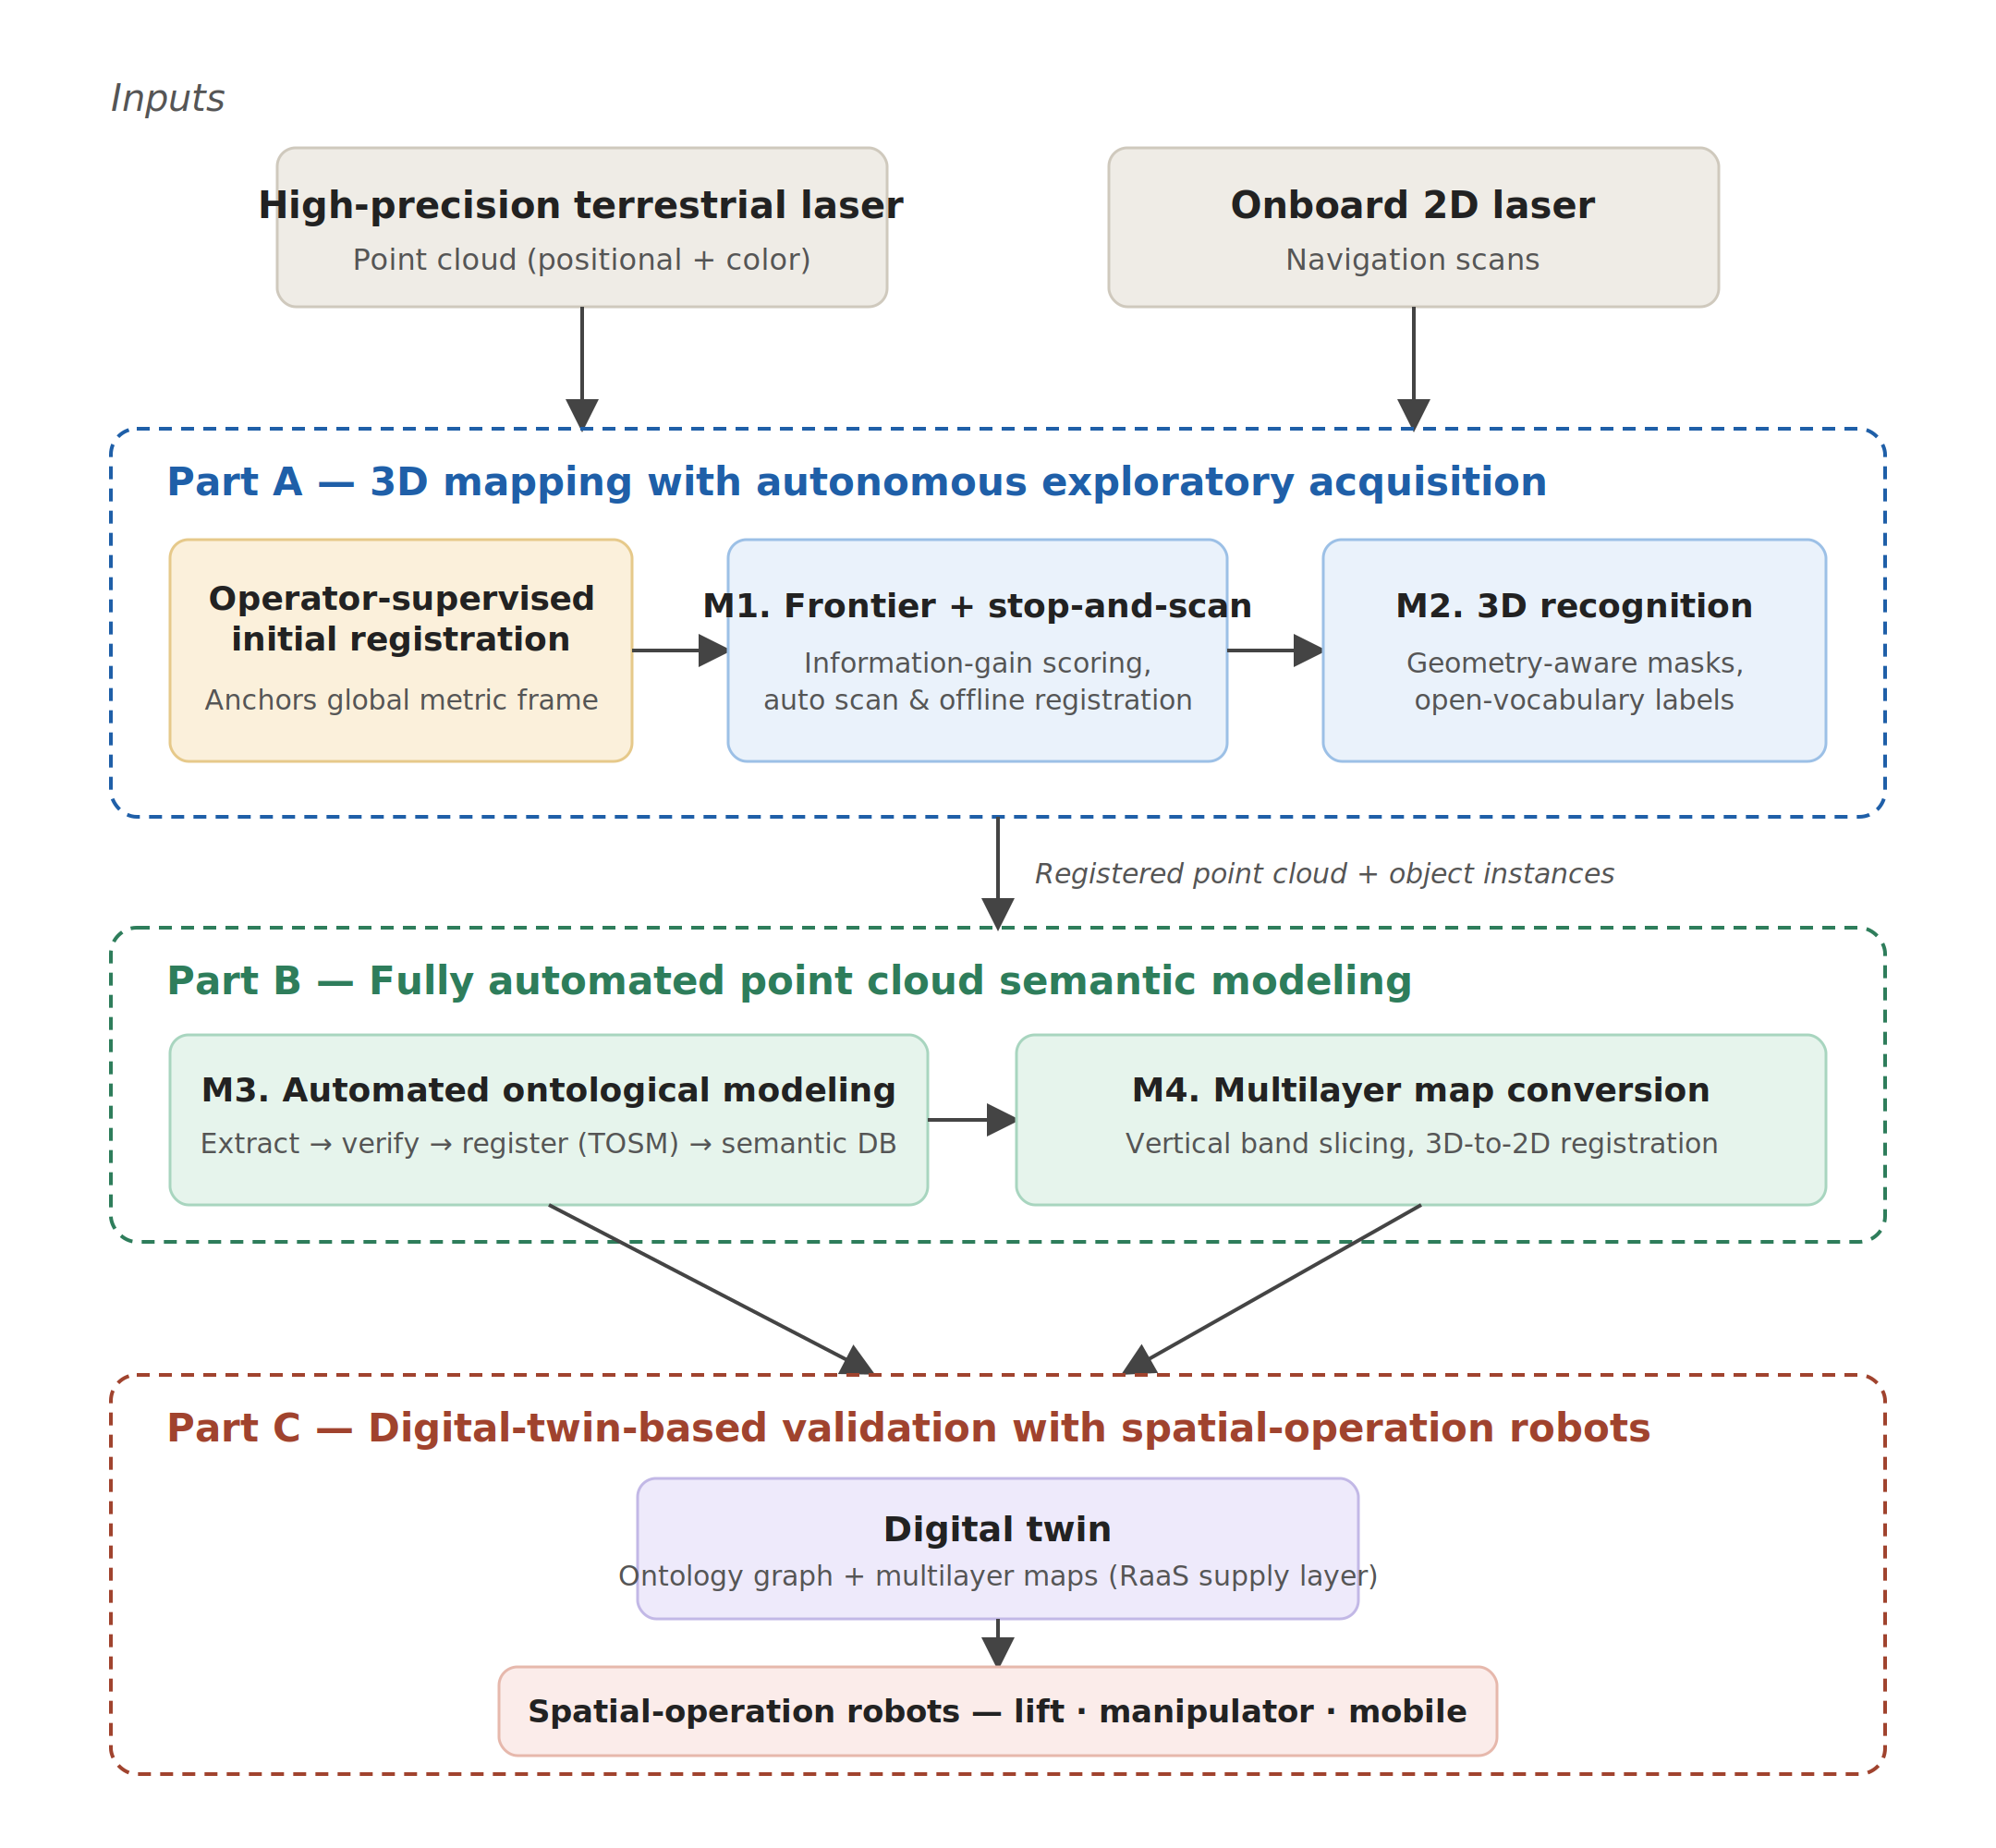
\includegraphics[width=0.95\textwidth]{figures/fig1_1.png}
  \caption{Overall structure of the proposed framework. Part~A performs 3D
  mapping with autonomous exploratory acquisition, Part~B performs fully
  automated point cloud semantic modeling, and Part~C performs
  digital-twin-based validation; a representation generated once by the mapping
  robot is shared and consumed by spatial-operation robots.}
  \label{fig:overall}
\end{figure}

\section{Publications}
\label{sec:publications}

The content of this dissertation has been published, accepted for presentation,
or submitted for publication in the following peer-reviewed venues, all with the author of this dissertation
as first author. Part~A (Chapter~\ref{ch:mapping} and
Section~\ref{sec:exp-mapping}) is based on the coverage-aware stop-and-scan
frontier exploration accepted for presentation at ICCAS~2026~\cite{iccas2026} and its journal
extension with the occlusion-aware visibility coverage model published in
\emph{Sensors}~\cite{kim2026sensors}. Part~B (Chapter~\ref{ch:semantic} and
Sections~\ref{sec:exp-seg}--\ref{sec:exp-ablation}) is based on the multi-view
VLM verification study accepted for presentation at ICTC~2026~\cite{kim2026ictc} and on the
TLS-driven semantic modeling framework (TLS-SMF) submitted to
\emph{Electronics}~\cite{kim2026electronics}. Part~C (Chapter~\ref{ch:validation}
and Sections~\ref{sec:exp-twin}--\ref{sec:exp-missions}) is based on the
automated scan-to-simulation pipeline accepted for presentation at RAAICON~2026~\cite{raaicon2026}
and on the application section of the \emph{Electronics} manuscript. The
knowledge-graph query lineage follows the ISIS~2025 work to which the author
contributed~\cite{kim2025isis}. Where text, tables, or figures are reused from
these publications, the source is indicated at the beginning of the
corresponding chapter.

\section{Dissertation Organization}
\label{sec:organization}

The remainder of this dissertation is organized as follows.
Chapter~\ref{ch:related} reviews related work on autonomous exploration and
coverage models, 3D semantic mapping and open-vocabulary recognition,
VLM-based verification and knowledge-grounded querying, incremental semantic-map
maintenance, and digital twins. Chapter~\ref{ch:mapping} details the automated
3D mapping subsystem: the stop-and-scan frontier exploration architecture, the
visibility-based coverage model, and the placement policy built on it.
Chapter~\ref{ch:semantic} describes the 3D point cloud semantic modeling
subsystem: the deterministic geometric backbone, multi-view VLM verification
with escalation, the TOSM schema and its serialization, identity matching and
confidence-gated update, corrective layers and owner feedback, structurally
gated querying, and the object-grounded place layer.
Chapter~\ref{ch:validation} presents the digital-twin-based validation
architecture: the scan-to-simulation pipeline, the live twin bridge, the
semantic mission stack, and the real-robot integration.
Chapter~\ref{ch:experiments} reports the experimental design and results for
all three parts. Chapter~\ref{ch:conclusion} concludes and discusses future
work.
